%!TEX root = ../my_thesis.tex
\chapter{Décodeurs polaires logiciels à Liste} % (fold)

% Intro chapitre

\vspace*{\fill}
\minitocTITI
\vspace*{\fill}
\newpage


\section{Introduction}

Le principe des réseaux mobiles cellulaires est de diviser le territoire en des zones appelées cellules. \`A chaque cellule est associé une station de base et un certain nombre de canaux de fréquence pour communiquer avec les terminaux mobiles. Chaque station de base est reliée aux différents réseaux gérant les appels vocaux et les messages textuels ainsi qu'à l'internet. Au fil de l'évolution des standards, la structure des réseaux mobiles cellulaires évolue, afin d'augmenter les performances de débit et de latence ainsi que le nombre de terminaux connectés. L'objectif est de faire face à la croissance exponentielle du nombre de terminaux.

La virtualisation des réseaux radio mobiles est considérée par les acteurs industriels \cite{ericsson_cloud_2015,huawei_5g:_2013} et académiques \cite{wubben_benefits_2014,rost_cloud_2014,checko_cloud_2015} comme une évolution prometteuse. Cette virtualisation est proposée en particulier pour les traitement effectués classiquement dans les stations de base. Comme illustré dans la Figure \ref{fig:bs}, dans les premières générations de téléphonie mobile (dites 1G et 2G), toutes les étapes de traitement du signal sont réalisées dans la station de base, à proximité de l'antenne. Une première évolution introduite dans les réseaux 3G est la séparation des traitements fréquence radio (RF : Radio Frequency) d'un coté et des traitements en bande de base (BB : Base Band) de l'autre. Comme représenté dans la Figure~\ref{fig:bbu}, chaque unité BB associée à chaque station de base est distante de l'antenne (jusqu'à 40 kilomètres). La connexion repose sur une liaison filaire. Dans ces unités BB sont réalisés les traitements numériques dont les étapes d'encodage et de décodage de canal. La cellule RF a pour rôle la conversion depuis la bande de base vers la bande RF. L'avantage de cette évolution est de pouvoir placer les infrastructures pour le traitement en BB près des centres urbains pour afin de faciliter la maintenance et de réduire les coûts.

Dans une structure de réseau de type Cloud-RAN (Cloud Radio Access Network), les ressources matérielles de calcul en BB sont partagées entre plusieurs antennes. Des optimisations sont ainsi rendues possibles : i) une meilleure adaptation aux trafics non uniformes, ii) des économies d'énergie, iii) des augmentations de débits et des réductions de la latence et enfin iv) une évolutivité et une maintenabilité accrues \cite{checko_cloud_2015}. Pour cela, les unités de traitement BB doivent être virtualisées. Il ne doit plus y avoir de support matériel dédié pour chaque station de base. Au contraire, les calculs doivent être distribués au niveau du Cloud. Pour ce faire, il est nécessaire que tous les algorithmes exécutés pour le traitement BB soient implémentés logiciellement. Le décodage de canal est une des tâches les plus intensives en calcul \cite{rodriguez_towards_2017,nikaein_processing_2015}. Il est donc primordial de disposer d'implémentations logicielles de décodeurs de canal qui soient à la fois efficaces et flexibles.

\begin{figure}[ht]
  \centering
  \subfloat[Stations de base traditionnelles]{
  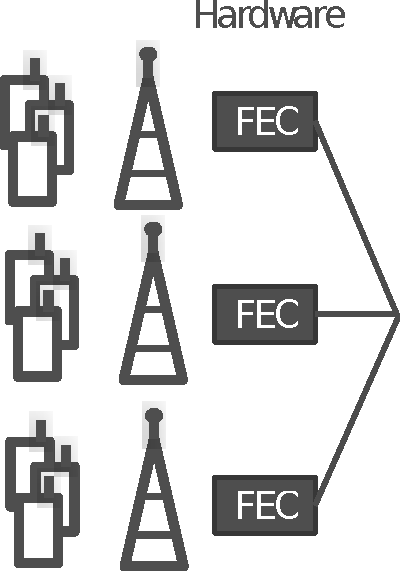
\includegraphics[scale=0.5]{main/ch2_fig/bs}
  \label{fig:bs}
  }
  \quad\quad
  \subfloat[Séparation BB / RF]{
  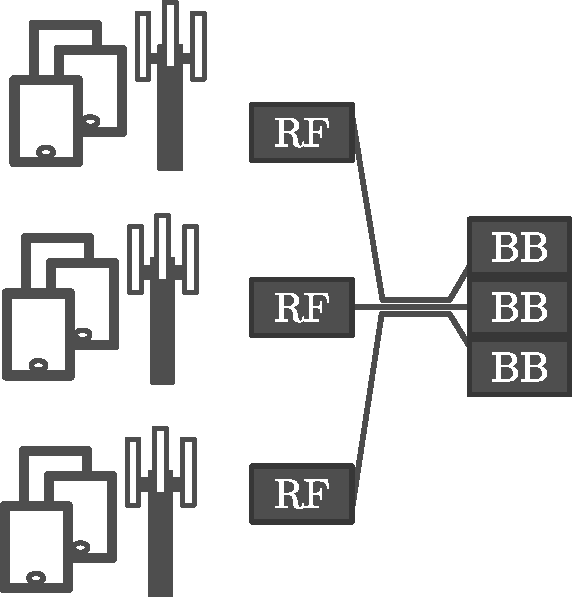
\includegraphics[scale=0.5]{main/ch2_fig/bs2}
  \label{fig:bbu}
  }
  \quad\quad
  \subfloat[Cloud-RAN]{
  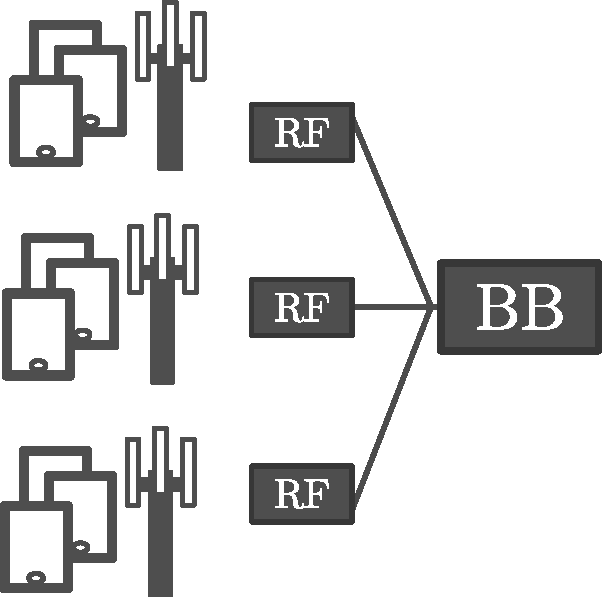
\includegraphics[scale=0.5]{main/ch2_fig/c-ran}
  \label{fig:c-ran}
  }
  \caption{\'Evolution de l'architecture des stations de base}
  \label{fig:bs_evo}
\end{figure}

Ce chapitre est divisé comme suit. Tout d'abord, la Section~\ref{sec:art_scl} présente l'état de l'art des implémentations logicielles de l'algorithme SCL sur des processeurs à usage général. Dans cette même section, nous présentons les principales techniques permettant d'atteindre de hauts débits et de faibles latences. 
Nous décrivons ensuite les implémentations proposées qui ont la propriété d'être flexibles et génériques. Dans un souci de clarté, la Section~\ref{sec:gen_scl} définit précisément ces concepts de généricité et de flexibilité qui sont au \coeur de l'étude. La Section \ref{sec:opti_scl} détaille les optimisations d'implémentation que nous proposons. Ces dernières permettent d'atteindre des débits et des latences compétitifs tout en conservant des caractères génériques et flexibles. Enfin, la Section~\ref{sec:exp_scl} compare les différentes implémentations proposées avec des implémentations de l'état de l'art.

\section{\'Etat de l'art portant sur les implémentations logicielles de l'algorithme SCL}
\label{sec:art_scl}
Les deux principales techniques d'implémentation logicielle permettant d'atteindre de hauts débits et de réduire la latence de décodage des codes polaires sont la vectorisation et le déroulage du code source. Cette section présente ces deux techniques d'implémentation logicielle.

\subsection{Vectorisation}

\begin{figure}
\lstset{language=C++,
        basicstyle=\footnotesize\ttfamily,
        keywordstyle=\bfseries\color{green!40!black},
        commentstyle=\itshape\color{purple!40!black},
        identifierstyle=\color{blue},
        stringstyle=\color{orange},
        morecomment=[l][\color{magenta}]{\#}
}
\begin{lstlisting}[language=C++, numbers=left, numbersep=0.3em, tabsize=2, basicstyle=\footnotesize\ttfamily]
class API_polar
{
  // l'usage de templates permet le support de différents formats
  // de données : virgule fixe, virgule flottante, nombre de bits
  template <typename R>
  // le type "Reg" permet l'accès aux registres vectoriels
  mipp::Reg<R> f_simd(const mipp::Reg<R> &la,
                      const mipp::Reg<R> &lb)
  {
    // toutes les opérations nécessaires aux fonctions polaires
    // sont vectorisées (abs, min, sign, neg)
    auto abs_la  = mipp::abs(la);
    auto abs_lb  = mipp::abs(lb);
    auto abs_min = mipp::min(abs_la, abs_lb);
    auto sign    = mipp::sign(la, lb);
    auto lc      = mipp::neg(abs_min, sign);

    return lc;
  }

  template <typename B, typename R>
  mipp::Reg<R> g_simd(const mipp::Reg<R> &la,
                      const mipp::Reg<R> &lb,
                      const mipp::Reg<B> &sa)
  {
    auto neg_la = mipp::neg(la, sa);
    // MIPP supporte également la surcharge d'opérateurs
    auto lc     = neg_la + lb;

    return lc;
  }

  \end{lstlisting}
  \caption{Implémentation logicielle des fonctions $f$ et $g$ utilisant la librairie MIPP.}
  \label{fig:mipp}
  \end{figure}

Les processeurs à usage général (GPPs : General Purpose Processors) actuels sont équipés d'unités de calcul vectoriel SIMD (Single Instruction Mutiple Data). Les architectures de processeurs x86-64 définissent par exemple des jeux d'instructions SIMD nommés SSE et AVX. Ces jeux d'instructions contiennent des opérations de chargement et de sauvegarde. Ces opérations permettent d'accéder aux données en mémoire et de les déplacer dans le fichier de registres. Ils intègrent également des opérations de calcul, comme les additions, soustraction ou multiplication.

Réduire le temps d'exécution des algorithmes de décodage de codes polaires à l'aide d'instructions SIMD est une technique classique utilisée dans de nombreuses implémentations de l'algorithme SC \cite{sarkis_fast_2014,giard_fast_2014,giard_low-latency_2016,sarkis_autogenerating_2014,gal_software_2014,cassagne_efficient_2015,cassagne_energy_2016,gal_multi-gb/s_2015} comme de l'algorithme SCL \cite{sarkis_fast_2016,sarkis_increasing_2014,shen_low-latency_2016}. Nous utilisons dans nos travaux une librairie générique et portable implémentant les fonctions élémentaires des codes polaires \cite{cassagne_efficient_2015}. Elle est basée elle-même sur la librairie MIPP \cite{cassagne2018mipp} qui est une encapsulation des instructions SIMD dont la description logicielle est écrite en langage C++.

L'utilisation de cette librairie présente plusieurs avantages. D'une part le code source apparaît clair, lisible et compact, contrairement à ce qui serait obtenu en utilisant un langage assembleur. Un extrait du code est donné dans la Figure~\ref{fig:mipp}. D'autre part, le code source est portable puisqu'il est compatible avec différentes cibles architecturales (Intel x86, Xeon KNL et ARM) à travers l'utilisation de différents jeux d'instructions (SSE, AVX et NEON). Enfin, MIPP permet d'utiliser plusieurs formats de représentation des données, à savoir : virgule flottante sur des mots de 32 ou 64 bits, virgule fixe sur des mots de 8, 16, 32 ou 64 bits. Plus le nombre de bits utilisés pour représenter une donnée est faible, plus le parallélisme résultant est important. Ainsi, le jeu d'instruction AVX2 permet de manipuler et de réaliser des opérations sur des registres de 256 bits. Si les données manipulées sont représentées sur 8 bits, alors le niveau de parallélisme et de 64. En clair, 64 opérations peuvent être alors réalisées en parallèle. Il est à noter que la versatilité de la librairie MIPP est obtenue sans perte de performance de décodage comme démontré dans \cite{cassagne2018mipp}.

Comme évoqué dans la Section \ref{subsubsec:parallel}, dans le contexte du décodage de codes polaires, il existe deux stratégies principales de parallélisation. Le parallélisme est utilisé soit pour décoder plusieurs trames en parallèle (\textit{inter-trame}), soit pour accélérer le décodage de chaque trame prise individuellement (\textit{intra-trame}). Dans les travaux présentés ici, seule la stratégie \textit{intra-trame} est utilisée. En effet cette dernière permet d'obtenir des latences plus faibles que dans le cas d'une stratégie \textit{inter-trame}. Le principe de la stratégie \textit{intra-trame} est d'appliquer simultanément plusieurs fonctions polaires élémentaires ($f$, $g$ ou $h$) sur un ensemble de données contenues dans un \noeud de l'arbre. Il est également possible d'utiliser des instructions SIMD pour réaliser les opérations sur les données contenues dans les feuilles. En effet, que ce soit dans les feuilles de type \texttt{R1}, \texttt{REP} ou \texttt{SPC}, il est nécessaire d'effectuer des opérations de seuillage sur un nombre de LLRs correspondant à la taille du \noeud. Ce seuillage est effectué en parallèle sur tous les LLRs du \noeud considéré grâce à des instructions SIMD.

Toutefois, le parallélisme \textit{intra-trame} n'est exploitable que dans la partie supérieure de l'arbre. \`A ce niveau, les \noeuds contiennent un nombre de données supérieur au niveau de parallélisme des unités SIMD. Dans le bas de l'arbre, près des feuilles, la librairie MIPP \cite{cassagne_efficient_2015} utilise automatiquement les versions séquentielles des implémentations des fonctions élémentaires. Dans le cas de l'algorithme CASCL sur un code polaire de taille (2048, 1723), l'augmentation du débit obtenu par l'utilisation des instructions AVX2 sur un processeur Intel i7 6600K est d'environ 20\% pour considérant les décodeurs proposés.


\subsection{Déroulage du code source}
\label{subsec:unroll}
La seconde technique classique que nous retrouvons dans les travaux récents est le déroulage du code source \cite{sarkis_autogenerating_2014,giard_fast_2014,cassagne_efficient_2015,cassagne_energy_2016}. Il découle de l'observation faite sur les décodeurs implémentant l'algorithme SC que les différents tests nécessaires au parcours de l'arbre de décodage prennent un temps significatif. Le parcours de l'arbre étant une donnée statique de l'algorithme de décodage, il est ainsi possible d'éviter ces tests en \og déroulant \fg le code source avant la compilation. La Figure~\ref{fig:unrolling} est une illustration de ce déroulage. D'un coté, dans le code non déroulé de la Figure \ref{fig:alg_rolled}, des appels récursifs potentiellement coûteux de la fonction \textit{DecodeNode} sont réalisés. De plus, des branchements conditionnels sont nécessaires pour traiter des feuilles de types différents (\texttt{R0}, \texttt{R1}, \texttt{REP} ou \texttt{SPC}). Au contraire, dans l'implémentation de la Figure~\ref{fig:alg_unrolled}, ni appel récursif ni branchement conditionnel ne sont nécessaires. Seules les fonctions élémentaires polaires sont appelées.

Il est à noter que l'arbre de décodage que nous prenons en exemple, dans la Figure~\ref{fig:unrolled_tree}, n'est pas élagué. Lors du décodage d'un arbre élagué, le nombre de tests effectués au cours du parcours de l'arbre augmente en proportion du nombre total d'instructions. Cela résulte du fait que le nombre de fonctions polaires différentes augmente. En effet, les fonctions \texttt{REP} et \texttt{SPC} sont ajoutées ainsi que des versions différentes des fonction $f$, $g$ et $h$ prenant en compte l'existence de \noeuds spécialisés dans l'arbre élagué, comme décrit dans \cite{sarkis_fast_2014,cassagne_efficient_2015}. Dans certains cas, le déroulage du code source permet d'augmenter jusqu'à un facteur 2 les débits de décodage \cite{sarkis_autogenerating_2014}. Cette technique de déroulage a été également étendue pour l'algorithme de décodageSCL \cite{sarkis_fast_2016}.

  \begin{figure}[t]
  \subfloat[Code non déroulé.]{
  \begin{minipage}{.35\linewidth}
  	\LinesNumberedHidden
    \begin{algorithm}[H]
      \SetAlgoLined
      \textit{DecodeNode}($\mathcal{N}_{0,0}$)\;
	  \SetKwProg{Fn}{Function}{}{}
	  \Fn{DecodeNode ($\mathcal{N}_{i,j}$)}{
	    \eIf{i<n}
	    {
	     $f(\mathcal{N}_{i,j})$\;
	     \textit{DecodeNode}($\mathcal{N}_{i+1,2j}$) \;
	     $g(\mathcal{N}_{i,j})$\;
	     \textit{DecodeNode}($\mathcal{N}_{i+1,2j+1}$) \;
	     $h(\mathcal{N}_{i,j})$\;
	    }
	    {
	      \eIf{$\mathcal{N}_{i,j}$\text est gelé}
	      {\texttt{R0}($\mathcal{N}_{i,j}$)\;}
	      {\texttt{R1}($\mathcal{N}_{i,j}$)\;}
	    }
      }
      \caption{Non Déroulé}%
    \end{algorithm}%
  \end{minipage}%
  \label{fig:alg_rolled}
  } 
  \quad\quad
  \subfloat[Code déroulé.]{
  \begin{minipage}{.16\linewidth}
    \LinesNumberedHidden
    \begin{algorithm}[H]
    \setstretch{1.045}
      \SetAlgoLined
	  $f(\mathcal{N}_{0,0})$\;
	  $f(\mathcal{N}_{1,0})$\;
	  \texttt{R0}($\mathcal{N}_{2,0}$)\;
	  $g(\mathcal{N}_{2,1})$\;
	  \texttt{R0}($\mathcal{N}_{2,1}$)\;
	  $h(\mathcal{N}_{1,0})$\;
	  $g(\mathcal{N}_{0,0})$\;
	  $f(\mathcal{N}_{1,1})$\;
	  \texttt{R1}($\mathcal{N}_{2,2}$)\;
	  $g(\mathcal{N}_{1,1})$\;
	  \texttt{R1}($\mathcal{N}_{2,3}$)\;
	  $h(\mathcal{N}_{1,1})$\;
	  $h(\mathcal{N}_{0,0})$\;
	  \mbox{}\\
      \caption{Déroulé}%
    \end{algorithm}%
  \end{minipage}%
  \label{fig:alg_unrolled}
  }
  \subfloat[Arbre décodé.]{
  \begin{minipage}{.35\linewidth}
  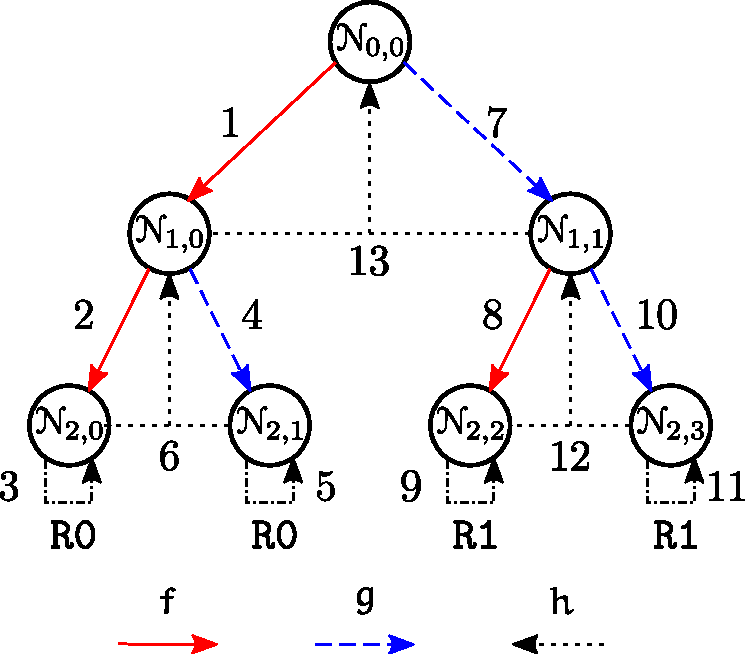
\includegraphics[width=\linewidth]{main/ch2_fig/unrolled_tree}
  \label{fig:unrolled_tree}
  \end{minipage}%
  }
  \caption{Déroulage du code source décrivant l'algorithme de décodage SC non élagué d'un code polaire (4,2) systématique.}
  \label{fig:unrolling}
\end{figure}

Les résultats d'implémentation logicielle au niveau des débits et latences des différents décodeurs reportés dans la littérature \cite{sarkis_increasing_2014,sarkis_fast_2016,shen_low-latency_2016} sont récapitulés et discutés dans la section \ref{sec:exp_scl}, dans le tableau \ref{tab:res} accompagnés des résultats des décodeurs proposés.

\section{Généricité et flexibilité d'un décodeur de codes polaires}
\label{sec:gen_scl}

\subsection{Définitions}
Les termes de généricité et de flexibilité pouvant donner lieu à diverses interprétations, nous proposons d'en donner une définition pour éviter toute ambiguïté.
Nous parlerons de la \textit{généricité} comme étant la capacité d'un décodeur à supporter n'importe quel encodage.
En effet, dans le contexte de communications mobiles, les paramètres de l'encodeur changent constamment pour s'adapter au canal. Pour ce faire, des méthodes adaptatives de modulation et de codage \cite{dahlman_4g:_2013} (AMC : Adaptive Modulation and Coding) sont appliquées. Ainsi, la taille du code polaire, le rendement de codage ou bien encore la position des bits gelés peuvent varier d'une trame à une autre. Par ailleurs, des patrons de poinçonnage sont souvent nécessaires. Enfin, des codes CRC sont concaténés aux codes polaires afin de détecter les erreurs et permettre des méthodes de transmission à demande de répétition automatique (ARQ : Automatic Repeat reQuest) ou leur évolution hybride (HARQ : Hybrid ARQ). Un décodeur générique devrait donc supporter toutes les combinaisons possibles de chacun de ces paramètres.

D'autre part, le terme \textit{flexibilité} s'appliquera au paramétrage de l'algorithme et des méthodes d'implémentation du décodeur, indépendamment du schéma de codage. Ces paramètres ne sont généralement pas imposés par le standard. Dans le cas de l'algorithme SCL, les paramètres suivants sont concernés : les variantes de l'algorithme (FASCL, PASCL), le format de représentation des données (virgule flottante ou fixe, nombre de bits), la taille de la liste $L$ ou encore l'élagage de l'arbre de décodage. La flexibilité du décodeur amène des degrés de liberté à l'implémentation permettant des compromis entre performances de décodage, latence et débit, pour un schéma d'encodage donné.

Comme nous allons le détailler dans les sections suivantes, tous les paramètres de généricité et de flexibilité cités sont supportés dans les implémentations de décodeurs proposées. Ils sont déterminés de manière dynamique à l'aide de fichiers de configuration ou des arguments de ligne de commande, lus lors de l'exécution. Aucune compilation du code source n'est nécessaire en cas de changement d'un paramètre. De ce choix découle le fait que nous n'utilisons pas la technique de déroulage présentée dans Section \ref{subsec:unroll}. En effet, cette technique implique la génération d'un code source pour chaque combinaison de paramètres comme proposé dans \cite{sarkis_autogenerating_2014} pour l'algorithme SC.

\subsection{Généricité}

\begin{figure}[t]
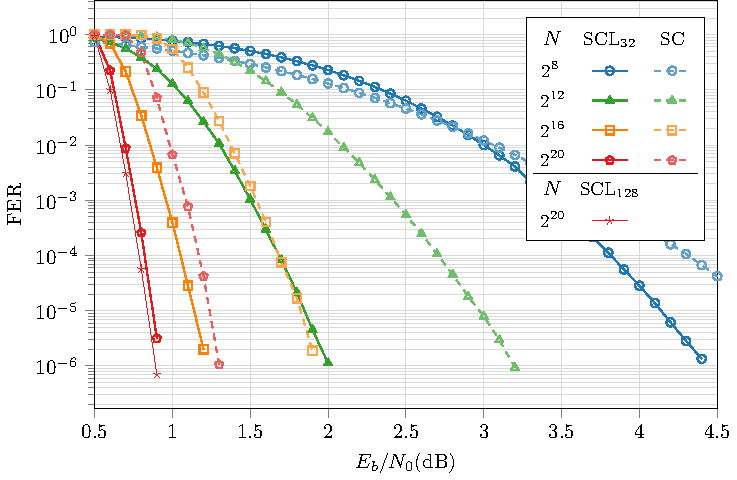
\includegraphics[width=\textwidth]{main/ch2_fig/curves/code/tikz/code}
\caption{Performances de décodage des algorithme SC et CASCL pour des très grandes tailles de code, $R=1/2$, CRC $c=32$ (GZip)}
\label{fig:large_scl}
\end{figure}

Les implémentations logicielles de décodeur proposées adressent n'importe quelle taille de mot de code. De plus, les débits des décodeurs étant compétitifs, il est possible d'explorer de grandes tailles de code conjointement à des profondeurs de liste importantes, comme montré dans la Figure~\ref{fig:large_scl}. Dans ce cas, $N$ prend des valeurs allant de $2^8$ à $2^{20}$ et le rendement du code polaire est $R=1/2$. Le CRC utilisé est défini dans le standard GZip : sa longueur est $c=32$ et son polynôme \texttt{0x04C11DB7}. 
Des simulations des performances de décodage de l'algorithme CASCL pour des codes polaires de grande taille ($N \geq 2^{14}$) sont rares dans la littérature. La seule référence disponible présente les performances de décodage de l'algorithme CASCL pour un code polaire ($32768$,$29504$) avec $L=4$.
L'algorithme SCL a été proposé pour améliorer les performances de décodage des codes polaires pour de petites tailles ($N<2^{12}$). Néanmoins, le fort débit du décodeur logiciel proposé permet de montrer que son utilisation pour des codes polaires de grande taille apporte également un gain significatif au niveau des performances de décodage. Dans le cas où $N=2^{12}$, l'utilisation de l'algorithme CASCL avec une taille de liste $L=32$ apporte un gain d'environ 1.2 dB lorsque le FER est égal à $10^{-5}$. Cependant, ce gain diminue lorsque $N$ augmente : 0.75 dB pour $N=2^{16}$ et 0.5 dB pour $N=2^{20}$. Des simulations ont également été réalisées pour une profondeur de liste $L=128$. Elles montrent que le gain par rapport à $L=32$ n'est pas significatif.

\subsection{Flexibilité}
Les paramètres de flexibilité sont eux aussi configurables lors de l'exécution du programme. Ils permettent divers compromis entre la latence, le débit et les performances de correction. Ainsi, l'algorithme de décodage peut être ajusté pour un code polaire donné. Dans la suite de cette section, ces paramètres de flexibilité sont détaillés et leurs effets analysés.

\subsubsection{Profondeur de la liste}
\begin{figure}[t]
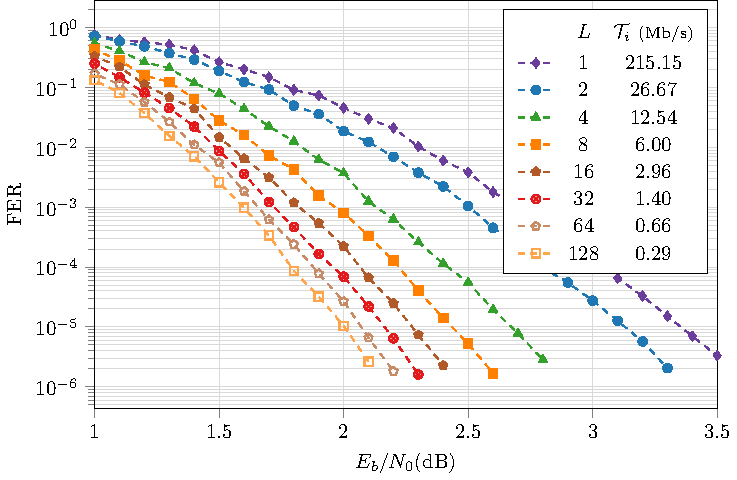
\includegraphics[width=\textwidth]{main/ch2_fig/curves/L/tikz/L}
\caption{Performances de décodage et débits de l'algorithme CASCL pour différentes valeurs de $L$ d'un code polaire ($2048,1024$) concaténé à un CRC $c=32$ (GZip).}
\label{fig:scl_l_thr}
\end{figure}
La profondeur de la liste impacte directement le pouvoir de correction et la complexité calculatoire de l'algorithme. La Figure~\ref{fig:scl_l_thr} représente les performances au niveau FER et les débits obtenus pour l'algorithme de décodage CASCL d'un code polaire ($2048$,$1024$). La complexité calculatoire augmente linéairement. Le débit est divisé approximativement par deux lorsque la profondeur de liste $L$ est doublée. Le seul cas ne respectant pas cette tendance est celui pour lequel $L=1$ qui correspond à l'algorithme SC. Ce dernier est bien plus rapide puisqu'il ne nécessite pas d'effectuer les calculs associés à l'algorithme SCL comme le tri, la génération des candidats, le calcul du CRC. Le FER évolue également avec $L$. \`A partir de $L\geq4$ et $E_b/N_0=2dB$, les performances au niveau FER diminuent continûment, de $4.10^{-3}$ à $10^{-5}$.

\subsubsection{Paramétrage fin de l'élagage}
L'élagage tel que défini dans la Section~\ref{subsec:pruning} est paramétrable très finement dans les implémentations de décodeurs polaires proposées. Tout d'abord, chaque type de \noeud (\texttt{R0}, \texttt{R1}, \texttt{REP} et \texttt{SPC}) peut être activé ou désactivé séparément. Cette caractéristique est utile pour analyser l'impact de l'utilisation de chaque type de \noeud sur le débit de décodage.

\`A ce stade, il est important de faire la distinction entre le débit codé et le débit d'information. Soit $\mathcal{T}_F$, le nombre de mots de code décodées par seconde. Dans ce cas, la valeur du débit d'information est $\mathcal{T}_i=K\mathcal{T}_F$, soit le nombre de bits d'informations décodés par seconde, tandis que la valeur du débit codé est $\mathcal{T}_c=N\mathcal{T}_F$.

Pour explorer l'impact de l'utilisation des types de \noeuds sur le débit, il apparaît plus pertinent d'utiliser le débit codé. En effet, si le débit d'information était utilisé dans la Figure~\ref{fig:nodes}, le rendement du code \og biaiserait \fg les débits. En effet, les débits des codes à haut rendement seraient supérieurs à ceux des codes à faible rendement.
\begin{figure}[t]
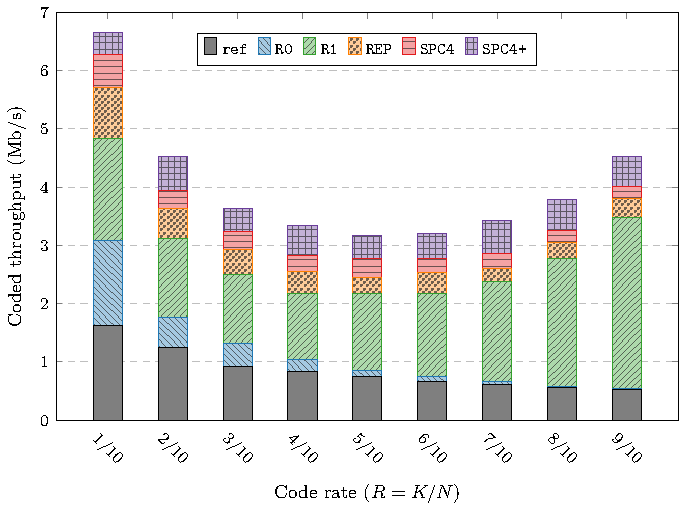
\includegraphics[width=\textwidth]{main/ch2_fig/curves/tree/tikz/tree}
\caption{Impact de l'activation des \noeuds d'élagage de l'algorithme CASCL, $N=2048$, $L=32$, $c=32$.}
\label{fig:nodes}
\end{figure}

\begin{figure}[t]
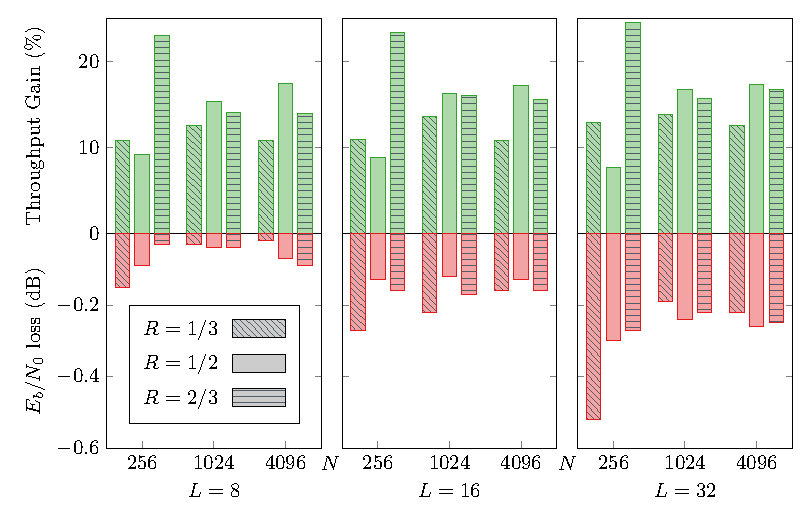
\includegraphics[width=\textwidth]{main/ch2_fig/curves/thr_spc/tikz/thr_spc_diff}
\caption{Effets de l'utilisation des \noeuds \texttt{SPC4+} dans l'algorithme CASCL pour un FER de $10^{-5}$}
\label{fig:spc_impact}
\end{figure}

Le débit codé de l'algorithme non élagué (\texttt{ref}) diminue lorsque le rendement augmente. Cela s'explique par le fait que les feuilles de rendement 1, plus nombreuses dans des codes à haut rendement, nécessitent plus de temps pour être décodées que les feuilles de rendement 0. En effet, dans l'algorithme SCL, le traitement d'une feuille de rendement 0 correspond à la mise à jour de métriques. Par ailleurs, le traitement d'une feuille de rendement 1 correspond à la génération de candidats, la mise à jour de leurs métriques, le tri de celles-ci et à des duplications d'arbres de décodage.

Dans la Figure \ref{fig:nodes}, les aires hachurées en diagonales (\raisebox{-\mydepth}{
\includegraphics[height=\myheight]{main/ch2_fig/hach1}},\raisebox{-\mydepth}{
\includegraphics[height=\myheight]{main/ch2_fig/hach2}}) représentent l'amélioration des performances de décodage lorsque les \noeuds \texttt{R0} et \texttt{R1} de tailles supérieures à un sont utilisés pour l'élagage. De manière attendue, l'élagage \texttt{R1} favorise une augmentation plus significative du débit pour les codes à haut rendement. Inversement, l'élagage \texttt{R0} s'avère plus efficace pour des codes à faible rendement. Une même tendance est observée pour l'élagage des \noeuds \texttt{REP}. Ces derniers sont plus efficaces pour des codes de faibles rendements. En effet, les \noeuds \texttt{REP} sont plus abondant dans les codes à faible rendements. En revanche, la tendance est moins claire pour les \noeuds \texttt{SPC}.

Il fut également observé dans \cite{sarkis_fast_2014} que lorsque la taille des \noeuds \texttt{SPC} n'est pas limitée à 4, les performances de décodage peuvent être dégradées. Dans les implémentations logicielles proposées, le choix a été fait de donner la possibilité de paramétrer finement la taille des \noeuds activés pour chaque type de \noeuds. En conséquence, leur taille est limitée à 4 dans les aires labellisées \texttt{SPC4} dans la Figure \ref{fig:nodes}. Les aires labellisées \noeuds \texttt{SPC4+} correspondent aux débits atteint lorsque le taille des \noeuds \texttt{SPC} n'est plus limitée à 4.

Dans nos expérimentations, la dégradation au niveau des performances de décodage due à l'utilisation des \noeuds \texttt{SPC4+} n'est pas systématique mais dépendante des caractéristiques du code polaire considéré. La Figure~\ref{fig:spc_impact} illustre le compromis entre le débit du décodeur et les performances de décodage lorsque les \noeuds \texttt{SPC4+} sont utilisés. La partie supérieure représente le débit du décodeur et la partie inférieure indique la dégradation induite pour les différents codes polaires considérés. Les augmentation de débits sont comprises entre 8\% et 20\% selon les cas, c'est-à-dire selon la profondeur de la liste, de la taille du mot de code et du rendement. La partie inférieure de la Figure \ref{fig:spc_impact} illustre pour sa part la dégradation des performances de décodage. Pour une profondeur de liste $L=8$, en dehors d'une configuration particulière ($N=256$, $R=1/3$), la dégradation du SNR pour un FER de $10^{-5}$ est inférieure à 0.1 dB. Si $L=32$ alors la dégradation est généralement légèrement supérieure à 0.2 dB. Encore une fois le cas du code polaire ($N=256$, $R=1/3$) est problématique, avec une dégradation d'environ 0.5 dB.

En conclusion, l'élagage de l'arbre permet des augmentations significatives du débit des décodeurs logiciels de l'algorithme SCL. Toutefois le traitement des \noeuds \texttt{SPC4+} décrit dans \cite{sarkis_fast_2016} peut provoquer une dégradation des performances de décodage qui dépend des paramètres de l'algorithme. Des tests complémentaires seraient nécessaire pour quantifier exhaustivement leur impact. La forte généricité et la grande flexibilité du décodeur logiciel proposé facilitent l'exploration de ce compromis entre performance de décodage et débit. Il est important de noter que l'activation des \noeuds d'élagage est effectué dynamiquement. Aussi, il serait possible de développer un décodeur logiciel qui adapterait dynamiquement son élagage, en temps réel, en fonctions des contraintes systèmes.

\subsubsection{Représentation en virgule fixe}

Il existe deux formats de représentation des nombres en base 2 : la représentation en virgule flottante et la représentation en virgule fixe. La représentation en virgule flottante offre une plus grande dynamique. Quant à la représentation en virgule fixe, elle simplifie simplifie les opérations arithmétiques. L'avantage des décodeurs de canal est que les données manipulées sont des données de type probabiliste. \`A ce titre, ces algorithmes sont souvent robustes vis-à-vis d'une diminution du nombre de bits utilisés pour représenter les données et par conséquent d'une représentation en virgule fixe.
L'avantage de représenter les données à l'aide d'un nombre réduit de bits et que cela permet aux unités SIMD d'effectuer davantage d'opérations en parallèle. 
L'objectif est donc de réduire le nombre de bits afin d'augmenter le parallélisme et par conséquence les performances de débit et de latence.

Des implémentations logicielles quantifiées de l'algorithme SC ont déjà été proposées \cite{giard_low-latency_2016} dans la littérature.
 Cependant, les décodeurs proposés constituent, à la connaissance de l'auteur, la première implémentation logicielle de l'algorithme SCL permettant de représenter les LLRs et les métriques de chemin sur 8 ou 16 bits.
Pour que la représentation en virgule fixe n'introduise pas de dégradation, des précautions doivent être prises.
Tout d'abord, pour des représentations sur 8 bits, les LLRs et les métriques de chemin sont saturées entre -127 et +127 après chaque opération.
De plus, les métriques de chemin sont normalisées après chaque opération de duplication et de sélection de candidats. Cela signifie que la valeur la plus faible des métriques de chemin est soustraite à chacune d'entre elles.
La Figure~\ref{fig:bfer_rep} montre les performances de l'algorithme CASCL pour différentes représentations des LLRs : 8 bits à virgule fixe, 16 bits à virgule fixe et 32 bits à virgule flottante.
Les courbes pour 32 bits et 16 bits sont confondues et montrent que la représentation sur 16 bits ne dégrade pas les performances. En revanche, des dégradations apparaissent pour la courbe pour 8 bits, labellisée \texttt{REP2+}.
Après analyse, il s'avère que ces dégradations sont dues au décodage des \noeuds de répétition.
En effet, lors de ce traitement, comme détaillé en Section \ref{subsec:pruning}, il faut sommer tous les LLRs du \noeud considéré.
Or pour un \noeud de répétition de grande taille, cette addition sur 8 bits peut induire un débordement.
La Figure \ref{fig:bfer_rep} montre que lorsque les \noeuds de répétition de taille supérieure à 8 sont désactivés (\texttt{REP8-}), ces débordements n'ont plus lieu et les performances sont similaires à celles d'un décodage effectué au format 32 bits à virgule flottante.

\begin{figure}
\centering
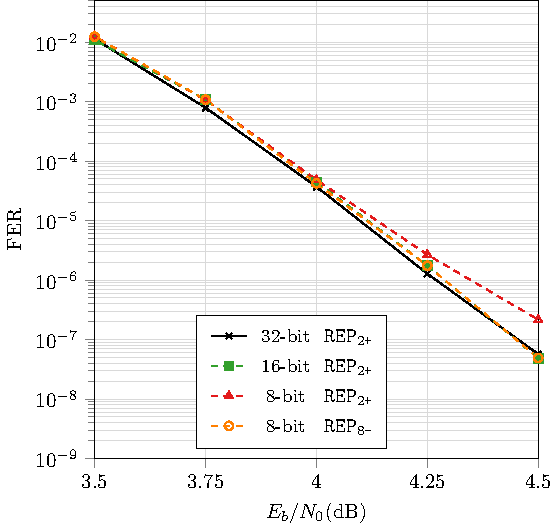
\includegraphics{main/ch2_fig/curves/bfer/tikz/bfer_rep}
\caption{Impact de l'utilisation des \noeuds de répétition sur des implémentations quantifiées.}
\label{fig:bfer_rep}
\end{figure}
  \begin{table}[b]
    \renewcommand{\arraystretch}{1.1}
    \centering
    \caption{Comparaison de débits et latences des algorithmes SCL adaptatifs pour des représentations à virgule flottante (32 bits) et virgule fixe (16 et 8 bits). Code polaire ($2048$,$1723$), $L=32$, CRC $c=32$ (GZip)}
    \label{tab:quantif}
    {\small\resizebox{\linewidth}{!}{
    \begin{tabular}{r | c | c || c | c || c | c || c | c}
      \multirow{2}{*}{\textbf{Décodeur}} & \multirow{2}{*}{\textbf{Quantif.}} & \multirow{2}{*}{$\bm{\mathcal{L}_{PC}}$} & \multicolumn{2}{c ||}{\textbf{3.5 dB}} & \multicolumn{2}{c ||}{\textbf{4.0 dB}} & \multicolumn{2}{c}{\textbf{4.5 dB}} \\
      \cline{4-9}
      & & & $\bm{\mathcal{L}_{moy}}$ & $\bm{\mathcal{T}_i}$ & $\bm{\mathcal{L}_{moy}}$ & $\bm{\mathcal{T}_i}$ & $\bm{\mathcal{L}_{moy}}$ & $\bm{\mathcal{T}_i}$ \\
      % \hline
      \hline
      \multirow{3}{*}{PA-SSCL} & 32-bit &  635 & 232.3 &   7.6 & 41.7 &  42.1 & 7.4 & 237.6 \\
      %\cline{3-9}
                               & 16-bit &  622 & 219.6 &   8.0 & 40.1 &  43.8 & 6.6 & 267.5 \\
      %\cline{3-9}
                               &  8-bit &  651 & 232.4 &   7.6 & 41.2 &  42.6 & 6.5 & 268.3 \\
      \hline
      \multirow{3}{*}{FA-SSCL} & 32-bit & 1201 &  67.2 &  26.1 &  8.5 & 207.8 & 5.1 & 345.5 \\
      %\cline{3-9}
                               & 16-bit & 1198 &  68.7 &  25.6 &  7.7 & 225.7 & 4.3 & 408.7 \\
      %\cline{3-9}
                               &  8-bit & 1259 &  71.8 &  24.4 &  7.7 & 227.3 & 4.1 & 425.9 \\
    \end{tabular}
    }}
  \end{table}

Dans le tableau \ref{tab:quantif} sont listés la latence \og pire cas \fg ($\mathcal{L}_{PC}$), la latence moyenne ($\mathcal{L}_{moy}$) et le débit d'information moyen ($\mathcal{T}_i$, en Mb/s) des algorithmes adaptatifs, PASCL et FASCL, pour les différentes représentations de l'information. Le processeur sur lequel les tests ont été réalisés est un processeur Intel i7 6600K. Dans le cas de la représentation sur 8 bits, les \noeuds répétitions de taille supérieure à 8 sont désactivés afin d'effectuer les mesures de vitesse pour performances de décodage identiques. Les représentations à virgule fixe réduisent dans la majorité des cas la latence moyenne, surtout dans les régions à fort SNR. Ceci est dû au fait que l'accélération apportée par la représentation en virgule fixe sur une nombre réduit de bits est plus importante pour l'algorithme SC que pour l'algorithme SCL. Or, dans le cas des algorithmes adaptatifs, plus le SNR est élevé, plus il est probable que le décodage SC suffise et qu'il n'y ait pas besoin de réaliser les décodages SCL. Ainsi, un débit de 425.9 Mb/s est atteint pour une représentation sur 8 bits des LLRs dans le cas de l'algorithme FASCL. Cela correspond à une augmentation de 80 Mb/s en comparaison avec la représentation sur 32 bits. Les décodeurs décrits montrent donc qu'il est possible d'implémenter les différents algorithmes à liste en représentant les données sur 8 bits sans dégrader les performances. Cette exploitation de la représentation en virgule fixe permet d'accélérer significativement le décodage des  implémentations logicielles des algorithmes à liste.

\begin{figure}[t]
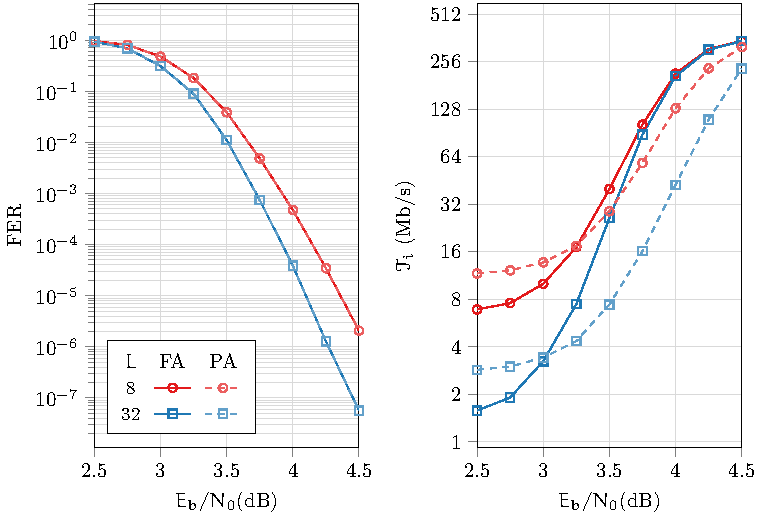
\includegraphics{main/ch2_fig/curves/ascl/tikz/ascl}
\caption{Performances de décodage et débits des algorithmes de décodage PASCL et FASCL pour un code polaire ($2048$,$1723$), $L=32$, et CRC $c=32$ GZip.}
\label{fig:ascl_perfs}
\end{figure}


\subsubsection{Les différentes variantes algorithmiques implémentées}
La Figure~\ref{fig:ascl_perfs} montre que les deux versions adaptatives de l'algorithme SCL, à savoir les algorithmes partiellement et complètement adaptatifs (PASCL et FASCL). Des débits différents sont observés suivant le rapport signal à bruit $E_b/N_0$ considéré. Pour de faibles valeurs de SNR, l'algorithme PASCL est plus avantageux. En revanche, l'algorithme FASCL prend l'avantage pour des valeurs intermédiaires, avant que les débits de chaque version se rapprochent pour les valeurs de $E_b/N_0$ les plus élevées.
L'explication de cette observation est la suivante : à faible SNR, la probabilité d'échec de décodage est très forte. La plupart du temps, l'algorithme adaptatif doit déclencher un décodage avec $L=L_{max}$ (ici $L_{max}=32$). Pour l'algorithme PASCL, dans ce cas précis où le décodage avec $L=32$ est nécessaire, deux décodages successifs seront déclenchés : le décodage SC puis le décodage SCL avec $L=32$. Pour l'algorithme FASCL, des exécutions intermédiaires de l'algorithme seront effectuées, pour $L=\{2,4,8,16\}$. En résumé, dans le cas le plus fréquent à faible SNR, l'algorithme PASCL est plus rapide que l'algorithme FASCL.
\`A fort SNR, le cas le plus probable est une réussite du décodage. Lorsque l'algorithme SC est suffisant pour décoder la trame, les algorithmes FASCL et PASCL auront des performances similaires. C'est pourquoi les débits des implémentations des deux algorithmes sont proches pour les valeurs les plus fortes de $E_b/N_0$. Pour des valeurs intermédiaires de SNR, le FASCL présente des débits supérieurs à ceux de l'algorithme PASCL. En effet, l'exécution de l'algorithme SCL avec des valeurs intermédiaires de $L$ est alors pertinent. Cependant, dans tous les cas et comme décrit dans la Section \ref{subsubsec:adaptive}, la latence \og pire cas \fg, autrement dit le temps maximum nécessaire pour le décodage d'une trame, est plus élevée pour l'algorithme FASCL. Ce fait est vérifié par la mesure comme reporté dans le Tableau~\ref{tab:quantif}.

La section \ref{sec:gen_scl} a permis de définir les concepts de généricité et de flexibilité du décodeur. Des contributions propres aux décodeurs proposés et liées à leur flexibilité ont également été introduites :

\begin{itemize}
  \item la représentation sur 8 et 16 bits en virgule fixe des données pour les algorithmes à liste,
  \item la configuration dynamique de l'élagage de l'arbre de décodage,
  \item le support de l'algorithme FASCL.
\end{itemize}

Cependant, ces implémentations doivent être compétitives par comparaison avec les décodeurs de la littérature du point de vue du débit et de la latence. Pour ce faire, des améliorations permettant d'atteindre de hauts débits et de faibles latences sont présentées dans la section suivante.

\section{Optimisations de l'implémentation logicielle des décodeurs à liste}
\label{sec:opti_scl}
Cette section \ref{sec:opti_scl} présente trois contributions originales. La première porte sur l'utilisation nouvelle d'un algorithme de tri des métriques et des LLRs. La seconde concerne l'accélération du contrôle de redondance cyclique. Enfin, la gestion des sommes partielles est l'objet d'une contribution propre.

\subsection{Algorithme de tri}
Des algorithmes de tri partiel sont appliquées durant de plusieurs étapes lors de l'exécution de l'algorithme SCL. Ainsi, les $L$ métriques de chemin les plus faibles doivent être identifiées pour sélectionner les candidats lors des étapes de duplication (étapes (i+1) et (i+3) de la Figure~\ref{fig:scl}). De plus, les 2 LLRs ayant les valeurs absolues les plus faibles doivent être identifiés lors du traitement des \noeuds \texttt{R1}. Enfin, les 4 LLRs les plus faibles doivent être retenus lors du traitement d'un \noeud \texttt{SPC}. 


Dans \cite{sarkis_fast_2016}, la méthode de tri des LLRs dans les \noeuds \texttt{REP} et \texttt{SPC} n'est pas précisée.
Schreier \cite{schreier_tournament_1932} donne un méthode pour identifier les deux plus petits (ou les deux plus grands) éléments d'un ensemble. Cette technique est également détaillée dans \cite{knuth_art_1973}. 
Il a été prouvé que cette méthode est la méthode optimale en termes de nombre de comparaisons deux-à-deux à effectuer.
Ce nombre est égal à $N+\log_2(N)-2$

\begin{figure}[t]
\centering
\subfloat[Identification du plus petit élément.]{
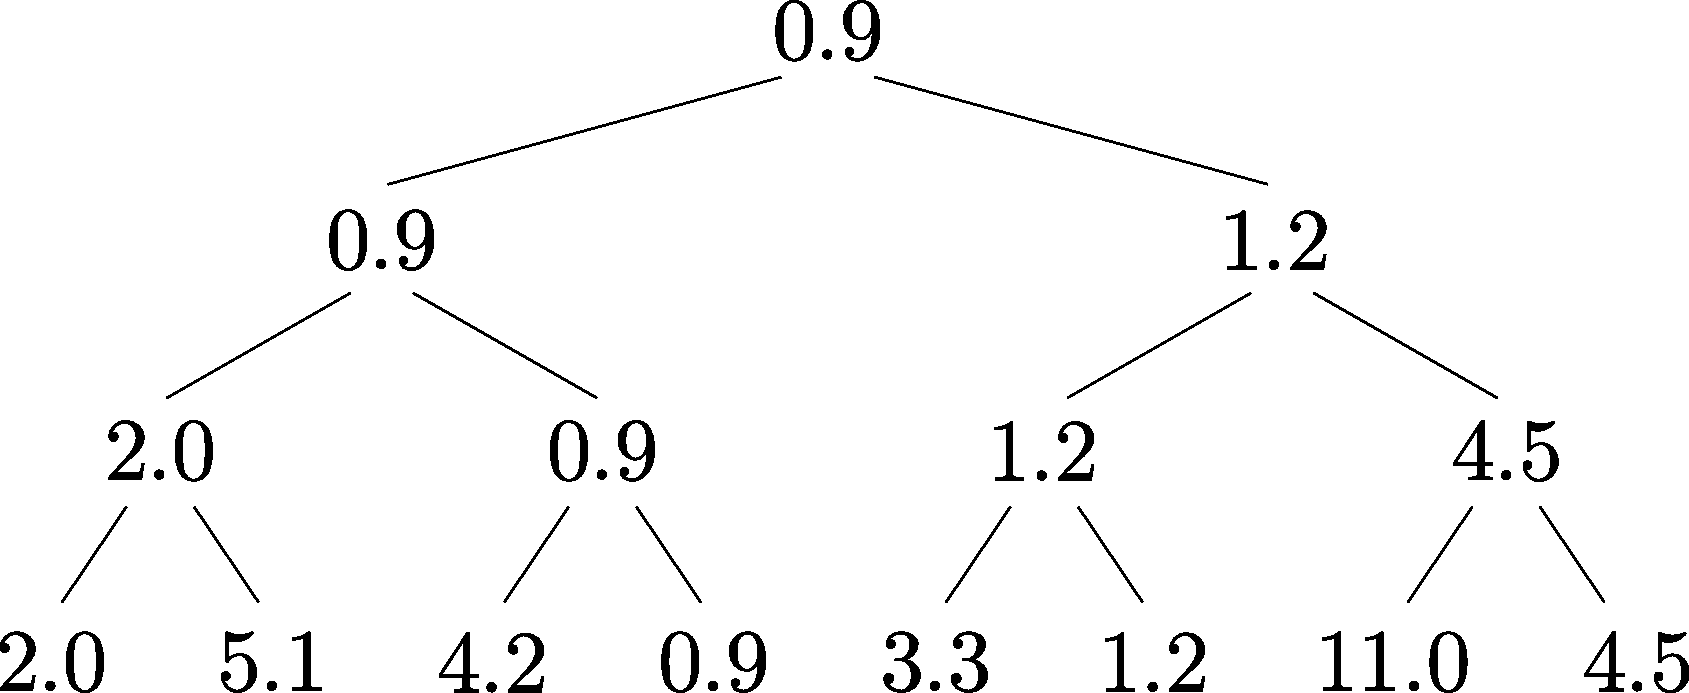
\includegraphics[width=0.75\textwidth]{main/ch2_fig/sorting_a}
\label{fig:sorting_a}
}
\\
\subfloat[Identification du second plus petit élément.]{
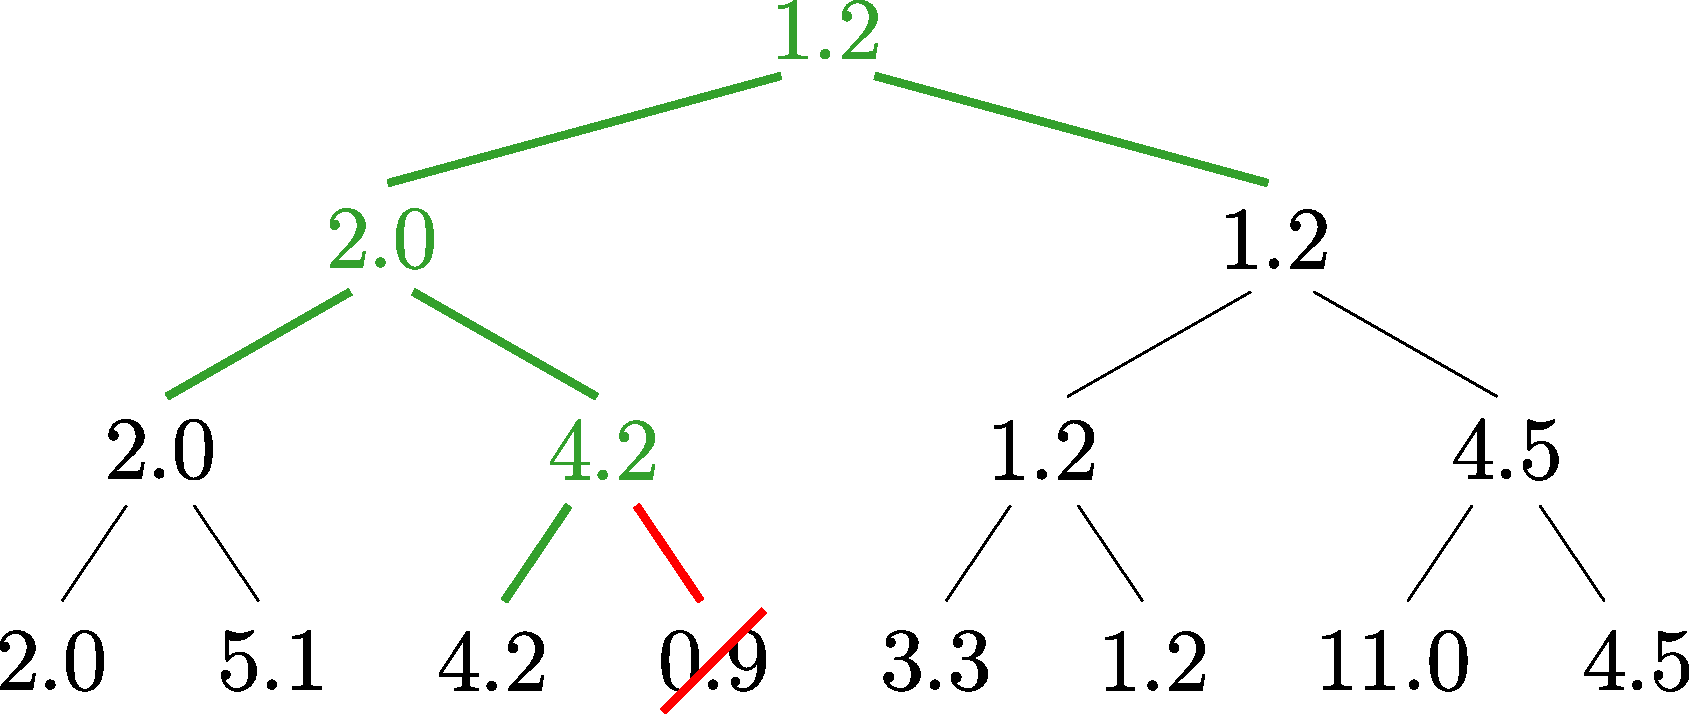
\includegraphics[width=0.75\textwidth]{main/ch2_fig/sorting_b}
\label{fig:sorting_b}
}
\caption{Méthode de Schreier}
\label{fig:schreier_sort}
\end{figure}
Elle nécessite deux étapes complémentaires, présentées en Figure~\ref{fig:schreier_sort}. La première étape est l'identification du plus petit élément par la traversée d'un arbre binaire. Durant la seconde étape, cet élément est éliminé, et la branche sur laquelle il se trouvait est rejouée. Le second élément le plus petit est ainsi identifié.


Cette méthode a été testée expérimentalement et ses performances ont été comparées à d'autres algorithmes potentiels : \textit{Batcher's merge exchange}, tri par bulle, tri \textit{quick-sort}, tri par tas implémenté dans la librairie standard. Les mesures ont été réalisées sur un processeur Intel i7 4790HQ, pour différents rendements, tailles de codes et profondeur de liste. La méthode de Schreier s'est révélé dans tous les cas le plus rapide. Elle l'était également dans les cas testés pour les \noeuds de type \texttt{SPC}. En effet, l'utilisation d'autres algorithmes de tri n'apporte pas de gain significatif.

Le tri des métriques dans \cite{sarkis_fast_2016} est effectué à l'aide d'un réseau de tri partiels (PSN : Partial Sorting Network) décrit dans []. Les unités de calcul SIMD sont utilisées pour accélérer l'exécution de ce tri. 
Dans un souci de simplicité de la description logicielle, le choix a donc été fait de n'utiliser que la méthode de Schreier pour réaliser les différents tris nécessaires pour l'exécution de l'algorithme SCL.
Dans cette étude, nous n'avons pas implémenté les PSN pour le tri des métriques. En effet, pour que ce réseau de tri soit générique vis à vis de $L$ ainsi que de l'élagage de l'arbre, une méthode devrait être conçue afin de créer un PSN pour n'importe quelle profondeur de liste $L$, et pour chaque type de \noeud différent. Nous pensons que l'utilisation de PSNs pourrait augmenter le débit de nos décodeurs. Toutefois, ce travail n'a pas encore été réalisé, et nous le réservons pour de futurs travaux.
Par défaut, la méthode de Schreier est également utilisée pour le tri des métriques. Les mêmes algorithmes alternatifs ont été testés mais aucune amélioration significative n'a permis d'amélioration du débit.

\subsection{Accélération du contrôle de redondance cyclique}

Par profilage de l'exécution d'un décodeur SCL adaptatif, il est possible d'observer que beaucoup de cycles d'exécution sont alloués aux vérifications de CRC.
En effet, durant chaque décodage (y compris le premier décodage SC), il est nécessaire de réaliser une vérification du CRC.
De plus, la complexité calculatoire d'une vérification de CRC est en $O(N)$ tandis que celle du reste de l'algorithme SCL est en $O(N\log N)$.
En conséquence, pour les valeurs de N considérées ($N<8192$), le temps nécessaire à la vérifications du CRC n'est pas négligeable vis à vis de celui nécessaire pour le décodage de code polaire proprement dit.

C'est pourquoi des méthodes d'implémentation efficaces doivent être utilisées afin de réduire le temps de vérification du CRC.
Pour ce faire, nous proposons que les bits soient empaquetés pour être traités 32 par 32.
\`A l'initialisation, les sommes partielles sont chacune stockées sur un entier.
Pour vérifier le CRC, 32 sommes partielles sont lues puis stockées dans un seul entier de 32 bits.
Une table de conversion est utilisée pour stocker des séquences calculées à l'avance du CRC.
La lecture de ces séquences permet de réduire la complexité calculatoire globale.

\begin{figure}[t]
  \centering
  \subfloat[Extraction séquentielle]{
  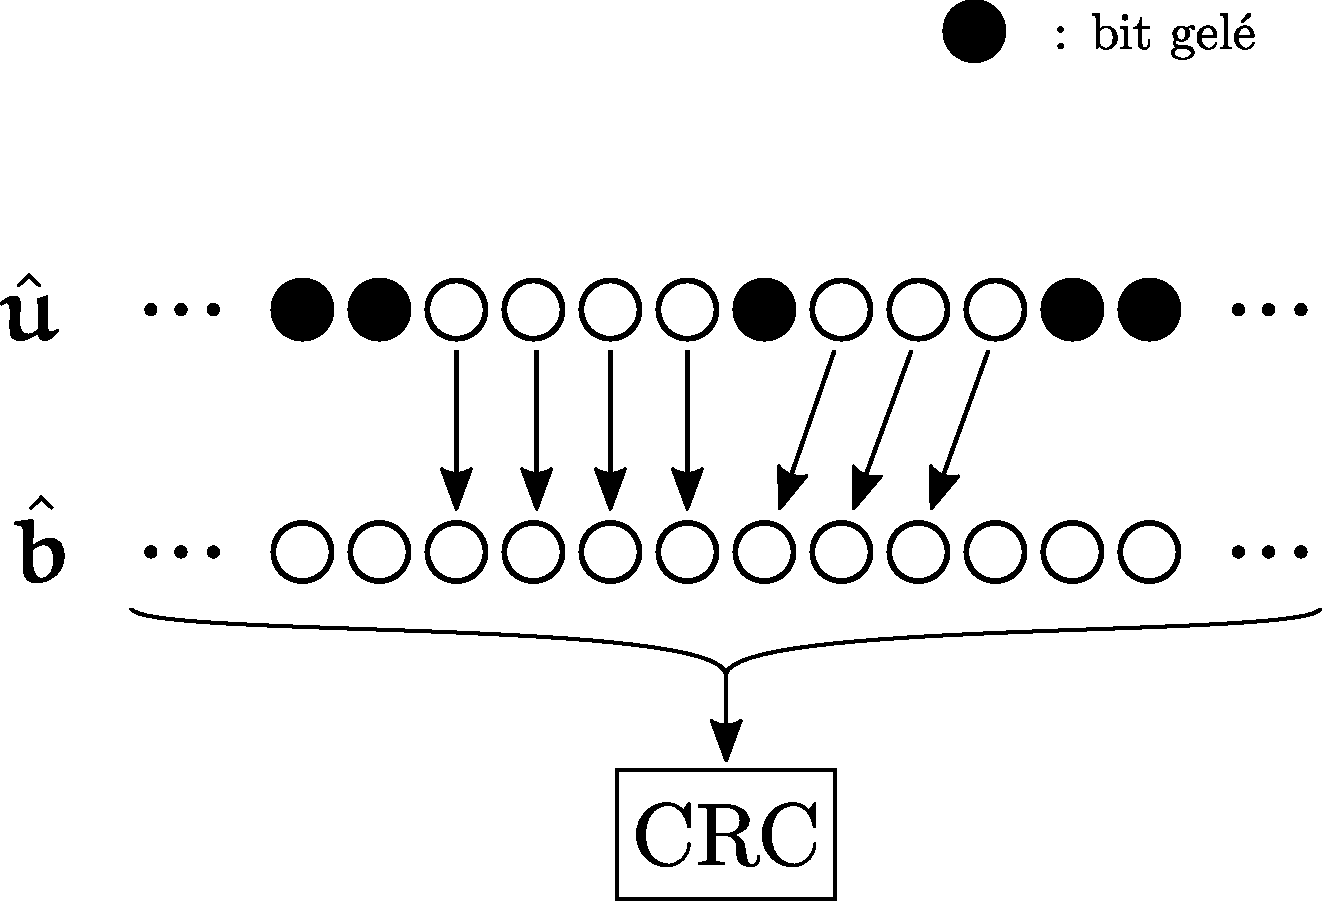
\includegraphics[height=120pt]{main/ch2_fig/extract1}
  \label{fig:extract1}
  }\quad
  \subfloat[Extraction parallèle]{
  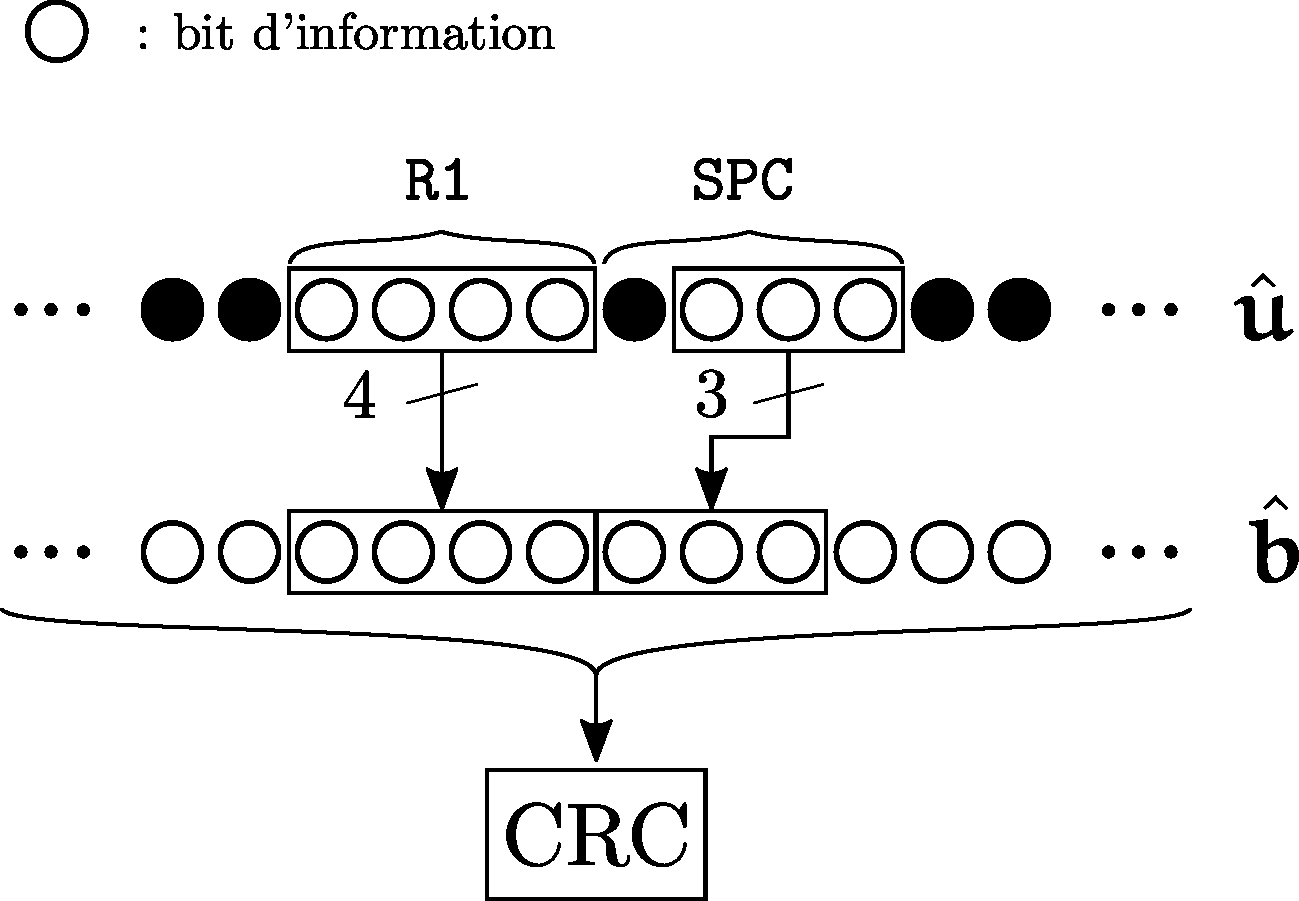
\includegraphics[height=120pt]{main/ch2_fig/extract2}
  \label{fig:extract2}
  }
  \caption{Extraction des bits d'information avant vérification du CRC}
  \label{fig:extract}
\end{figure}

Après chaque décodage SC ou SCL au sein des décodeurs adaptatifs, des mots de code candidats $\mathbold{\hat{u}}$ de $N$ bits sont produits.
Toutefois, le CRC est calculé sur les $K$ bits d'information de $\mathbold{\hat{b}}$ parmi les $N$ bits du mot de code.
Il est donc nécessaire de réaliser l'extraction des bits d'information.
L'implémentation naïve représentée dans la Figure~\ref{fig:extract1} consiste à réaliser cette extraction bit par bit.
Pour chaque bit, un test est réalisé pour savoir s'il s'agit d'un bit gelé ou d'un bit d'information.
Le profilage des décodeurs montre que cette opération d'extraction représente une portion non négligeable du temps total de traitement du CRC.
Or, il est possible de l'accélérer en utilisant la connaissance préalable de l'emplacement des bits gelés par la connaissance des \noeuds d'élagage.
En effet, la présence d'un \noeud de type \texttt{R1} de taille $4$ correspond à la présence de $4$ bits d'information consécutifs dans le vecteur $\mathbold{\hat{u}}$ comme représenté en Figure~\ref{fig:extract2}.
La fonction (\texttt{std::copy}) de la librairie standard C++ permet de réaliser une extraction parallèle de plusieurs bits.
CCette technique peut être étendue aux \noeuds \texttt{SPC} à condition d'exclure le bit gelé du \noeud en question.

Au cours de l'exécution des algorithmes adaptatifs, une vérification du CRC doit être effectuée une fois à la fin du décodage SC, et $L$ fois à la fin de chaque décodage SCL, afin de tester chaque candidat. En conséquence, l'accélération des vérifications de CRC est capital pour ces algorithmes adaptatifs.
Les mesures effectuées le vérifient. Pour l'algorithme FASCL sur un code polaire (2048,1723) associé un CRC de taille $c=32$ à $E_b/N_0 = 4.5dB$, le gain de performance d'exécution lié à l'utilisation des techniques présentées ci-dessus est de 63\%, portant le débit de 262 Mb/s à 426 Mb/s.

\subsection{Gestion des sommes partielles}
La gestion des sommes partielles dans les décodeurs proposés est détaillés dans cette sous-section.
Les sommes partielles sont des décisions dures. Cela signifie que leurs valeurs donc binaires. Cependant, dans les implémentations logicielles proposées, afin d'utiliser efficacement les instructions SIMD, les LLRs et les sommes partielles sont stockés sur des entiers de même dimension, notée $Q$, en octets. Selon la représentation choisie, 32, 16 ou 8 bits, $Q$ peut donc prendre respectivement les valeurs 4, 2 ou 1. 
Dans les précédentes implémentations logicielles de l'algorithme SCL \cite{sarkis_fast_2016,sarkis_increasing_2014,shen_low-latency_2016}, un emplacement mémoire de $Q$ octets est alloué à chaque niveau de l'arbre de décodage comme décrit dans \cite{tal_list_2011}. La taille de l'emplacement mémoire associé à un niveau de l'arbre est égal à la taille des \noeuds du niveau en question. Soit $n=\log_2(N)$, le nombre total de niveaux est $n+1$ et la taille d'un \noeud au niveau $l$ est égale à $2^{n-l}$. L'empreinte mémoire pour les sommes partielles d'un arbre de décodage est, quant à elle, égale à : 
\begin{equation}
\sum^n_{l=0}2^{n-l}=2N-1
\end{equation}
Pour l'algorithme SCL dans lequel L arbres de décodage sont nécessaires, l'empreinte mémoire totale est donc $L(2N-1)$. Cependant, dans l'algorithme SC, les sommes partielles d'un \noeud donné de l'arbre de décodage ne sont utilisées qu'une seule fois au cours du décodage. Par conséquent, ces emplacements mémoire peuvent être réutilisés. Ainsi, l'empreinte mémoire est réduite de $2N-1$ à $N$ dans l'algorithme SC \cite{leroux_hardware_2011}. De même, il est possible de réduire cette empreinte mémoire de $L(2N-1)$ à $LN$ pour l'algorithme SCL.

Lors des étapes de duplication et de sélection de l'algorithme SCL, étapes $(i+1)$ et $(i+3)$ de la Figure \ref{fig:scl}, il est nécessaire d'affecter les sommes partielles d'un arbre de décodage original à un nouvel arbre. Deux méthodes sont envisageables pour réaliser cette affectation. La première, notée $SCL_{cpy}$, consiste à systématiquement copier les $N$ sommes partielles sauvegardées dans l'emplacement mémoire du premier arbre de décodage vers l'emplacement mémoire du second. La seconde, présentée dans \cite{tal_list_2011}, est de réaliser cette affectation à l'aide de pointeurs. Ainsi, tant que les sommes partielles de chaque arbre ne diffèrent pas, ils utilisent le même emplacement mémoire. Cette méthode est notée $SCL_{ptr}$.

\begin{figure}
\centering
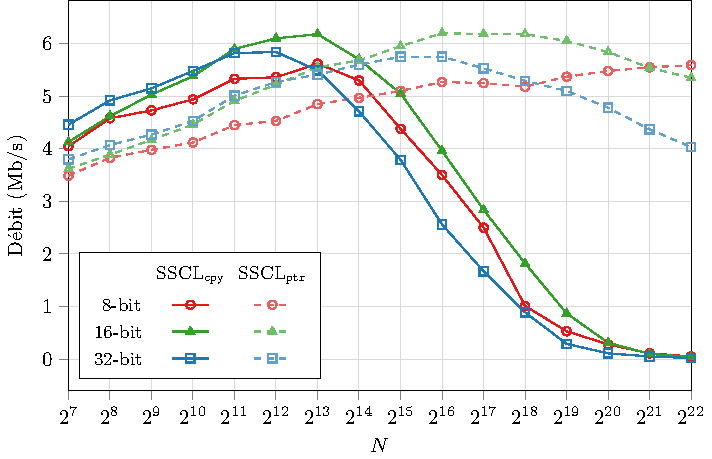
\includegraphics{main/ch2_fig/curves/thr/tikz/thr}
\caption{Comparaison des débits associés aux méthodes $SCL_{cpy}$ et $SCL_{ptr}$ pour différentes valeurs de $N$.}
\label{fig:scl_mem}
\end{figure}

La méthode $SCL_{ptr}$ semble plus efficace puisqu'elle évite des copies inutiles. Cependant, nos expérimentations ont montré que les calculs qui sont nécessaires à la gestion des pointeurs pénalisent cette méthode pour des codes de petite et moyenne tailles. La Figure~\ref{fig:scl_mem} représente les débits des implémentations de l'algorithme SCL associés aux deux méthodes, pour différentes valeurs de $N$, un rendement constant, $R=1/2$ et une profondeur de liste $L=32$. Ces courbes montrent que la méthode $SCL_{cpy}$ permet d'atteindre des débits plus élevés pour $N<8192$. En revanche, la méthode $SCL_{ptr}$ est plus avantageuse pour des tailles de codes supérieures. La Figure~\ref{fig:scl_mem} montre également l'impact du format utilisé pour la représentation des LLRs et des sommes partielles. Pour de très grandes valeurs de $N$, la représentation sur 8 bits est plus efficace, puisqu'elle occupe moins d'espace mémoire et que les échecs d'accès à la mémoire cache sont plus rares. 

Trois optimisations originales permettant d'augmenter le débit et de réduire la latence des implémentations des algorithmes de décodage de codes polaire à liste sont détaillées dans la Section \ref{sec:opti_scl} : nouvel algorithme de tri, accélération du traitement du CRC, et nouvelle méthode de gestion des sommes partielles.




\section{Expérimentations : mesures et comparaisons}
\label{sec:exp_scl}

Les débits et les latences des implémentations proposées sont détaillées dans cette section. Tous les résultats proposés ont été obtenus grâce à l'outil AFF3CT \cite{aff3ct_aff3ct:_2016}. Le code source de ce logiciel est ouvert et disponible en ligne. Ainsi, tous les résultats sont facilement reproductibles. La cible matérielle est un CPU Intel i5-6600K d'architecture Skylake. Le jeu d'instruction SIMD AVX2 est exploité. Sa fréquence pour les résultats reportés est 3.9 GHz. La compilation a été effectuée sur un OS Linux avec le compilateur C++ de GNU (version 5.4.0). Les options de compilation qui ont été appliquées sont les suivantes : \texttt{-Ofast -march=native -funroll-loops}.

\subsection{Algorithme complètement adaptatif}
L'algorithme FASCL permet d'atteindre les débits les plus élevés. Comme il est montré dans le Tableau~\ref{tab:quantif}, l'implémentation de cet algorithme avec une représentation sur 8 bits des LLRs et des sommes partielles permet d'atteindre un débit de 425 Mb/s pour un code polaire (2048,1723) et le CRC GZip de taille 32 bits lorsque $E_b/N_0=4.5dB$. Ce débit est pratiquement deux fois supérieur à celui obtenu avec l'algorithme PASCL. Le rapport signal à bruit pour lequel la différence entre PASCL et FASCL est la plus grande (380\%), est dans le domaine où le FER est compris entre $10^{-3}$ et $10^{-5}$. Il s'agit du domaine ciblé pour les communications sans fils comme le standard LTE ou le futur réseau 5G. Dans ces conditions, le débit de l'algorithme FASCL est d'approximativement 230Mb/s tandis que celui de PASCL est d'approximativement 40 Mb/s. Toutefois, rappelons que la latence dans le pire cas est plus élevée dans le cas de l'algorithme FASCL.

    \begin{table}[t]
      \centering
      \caption{Comparaison des débits et des latences des décodeurs proposés avec ceux de l'état de l'art. Représentation des LLRs et sommes partielles sur 32 bits. Code polaire (2048,1723), $L=32$, CRC GZip $c=32$.}
      \label{tab:res}
      {\small\resizebox{\linewidth}{!}{
      \begin{tabular}{r|l|c|c|c c c}
        \multirow{2}{*}{\textbf{Cible}} & \multirow{2}{*}{\textbf{Algorithme}} & \multirow{2}{*}{\textbf{Version}}  & \multirow{1}{*}{\textbf{$\bm{\mathcal{L}_{PC}}$}} & \multicolumn{3}{c}{$\bm{\mathcal{T}_i}$ (Mb/s)} \\
        \cline{5-7}
        &                        &   & ($\mu s$)                          & \textbf{3.5 dB} & \textbf{4.0 dB} & \textbf{4.5 dB} \\
        \hline
        % \hline
        i7-4790K & CASCL  & \cite{shen_low-latency_2016}      & 1572                           & 1.10            & 1.10            & 1.10            \\
        \hline
        i7-2600  & CASCL  & \cite{sarkis_increasing_2014}     & 23000                          & 0.07            & 0.07            & 0.07            \\
        i7-2600  & CASCL  & \cite{sarkis_fast_2016}           & 2294                           & 0.76            & 0.76            & 0.76            \\
        i7-2600  & CASCL  & Ce travail                        & 4819                           & 0.37            & 0.37            & 0.37            \\
        i5-6600K & CASCL  & Ce travail                        & 3635                           & 0.48            & 0.48            & 0.48            \\
        \hline
        i7-2600  & CASSCL & \cite{sarkis_increasing_2014}    & 3300                           & 0.52            & 0.52            & 0.52            \\
        i7-2600  & CASSCL & \cite{sarkis_fast_2016}          & 433                            & 4.0             & 4.0             & 4.0             \\
        i7-2600  & CASSCL & Ce travail                       & 770                            & 2.3             & 2.3             & 2.3             \\
        i5-6600K & CASSCL & Ce travail                       & 577                            & 3.0             & 3.0             & 3.0             \\
        \hline
        i7-2600  & PASSCL & \cite{sarkis_increasing_2014}    & $\approx$ 3300                 & 0.9             & 4.90            & 54.0            \\
        i7-2600  & PASSCL & \cite{sarkis_fast_2016}          & $\approx$ 433                  & 8.6             & 33.0            & 196.0           \\
        i7-2600  & PASSCL & Ce travail                       & 847                            & 5.5             & 31.1            & 168.4           \\
        i5-6600K & PASSCL & Ce travail                       & 635                            & 7.6             & 42.1            & 237.6           \\
        \hline
        i7-2600  & FASSCL & Ce travail                       & 1602                           & 19.4            & 149.0           & 244.3           \\
        i5-6600K & FASSCL & Ce travail                       & 1201                           & 26.1            & 207.8           & 345.5           \\
      \end{tabular}
      }}
    \end{table}

\subsection{Comparaison avec l'état de l'art}

Les débits et les latences des décodeurs proposés sont listés et comparés avec ceux de certains décodeurs de l'état de l'art dans le tableau \ref{tab:res}. Pour tous les décodeurs, les \noeuds SPC4+ ne sont pas utilisés afin de ne pas impacter les performances de décodage. La latence donnée dans le Tableau \ref{tab:res} est la latence \og pire cas \fg et le débit est le débit d'information moyen. La première version, CASCL, est l'implémentation de l'algorithme CASCL sans aucun élagage tandis que les versions notées CASSCL, FASSCL et PASSCL utilisent l'élagage de l'arbre. Le débit du décodeur CASSCL proposé (2.3 Mb/s) est seulement divisé par deux par comparaison avec l'implémentation spécifique déroulée de l'algorithme CASSCL décrite en \cite{sarkis_fast_2016} (4.0 Mb/s). Elle est approximativement 4 fois plus rapide que l'implémentation générique proposée en \cite{sarkis_increasing_2014} (0.52 Mb/s) et 2 fois plus rapide que celle proposée en \cite{shen_low-latency_2016}. Ce résultat est obtenu grâce aux améliorations algorithmiques proposées en Section \ref{sec:opti_scl}. De plus, les implémentations proposées présentent une flexibilité et une généricité bien plus grandes que celles proposées dans \cite{sarkis_increasing_2014,shen_low-latency_2016}. En effet, les représentations quantifiées, la possibilité de définir des patrons de poinçonnage et la possibilité d'utiliser les algorithmes adaptatifs n'étaient pas offertes. En utilisant la même cible matérielle (i7-2600), l'implémentation de l'algorithme PASSCL présente des débits proches de l'implémentation spécifique déroulée de \cite{sarkis_fast_2016}. Enfin, le débit obtenu pour l'algorithme FASSCL est lui bien meilleur (jusqu'à 244 Mb/s pour $E_b/N_0=4.5dB$).

\subsubsection{Performances sur différentes cibles matérielles}
  \begin{table}[t]
    \centering
    \caption{Comparaison des débits, du nombres de cycles d'horloge nécessaires pour décoder une trame, et de l'énergie dépensée par bit décodé, pour des décodeurs proposés sur différentes cibles matérielles. Représentation en virgule fixe sur 8 bits , $E_b/N_0 = 4.5dB$, CRC GZip $c=32$.}
    \label{tab:port}
    {\small\resizebox{\linewidth}{!}{
    \begin{tabular}{r|c|c|c c c c| c c c| c c c}
      \multirow{3}{*}{\centering \textbf{Target}}  & \multirow{3}{*}{\begin{minipage}{0.5in}\centering \textbf{Freq. (MHz)}\end{minipage}} & \multirow{3}{*}{\centering \textbf{Algo.}}  & & \multicolumn{3}{c|}{$\bm{\mathcal{T}_i}$ \textbf{(Mb/s)}} & \multicolumn{3}{c|}{\textbf{\# Cycles par trame}} & \multicolumn{3}{c}{$\bm{\mathcal{E}_b}$ \textbf{(nJ/bit)}} \\
      \cline{4-13}
       & & & & \textbf{3.5} & \textbf{4.0} & \textbf{4.5} & \textbf{3.5} & \textbf{3.5} & \textbf{3.5} & \textbf{3.5} & \textbf{4.0} & \textbf{4.5} \\
       & & & & \textbf{dB}  & \textbf{dB}  & \textbf{dB}  & \textbf{dB}  & \textbf{dB}  & \textbf{dB}  & \textbf{dB}  & \textbf{dB}  & \textbf{dB}  \\
      \hline
      \hline
      \multirow{3}{*}{\begin{minipage}{0.5in}\centering i7 4790\end{minipage}}     & \multirow{3}{*}{\begin{minipage}{0.5in}\centering 3592\end{minipage}} 
        & CASCL &                     &  2.34  & 2.38   & 2.24   & 2645 & 2600 & 2763 & 6325 & 6218 & 6607 \\
      & & PASCL &                     &  5.80  & 33.88  & 207.96 & 1067 & 183  & 30   & 2552 & 437  & 71   \\
      & & FASCL &                     &  19.43 & 194.66 & 372.30 & 319  & 32   & 17   & 762  & 76   & 40   \\

      \hline
      \multirow{3}{*}{\begin{minipage}{0.5in}\centering Ryzen 2700X\end{minipage}} & \multirow{3}{*}{\begin{minipage}{0.5in}\centering 4230\end{minipage}} 
        & CASCL &                     &  2.68  & 2.72   & 2.56   & 2675 & 2635 & 2800 & 5149 & 5074 & 5391 \\
      & & PASCL &                     &  6.55  & 38.76  & 237.78 & 1094 & 185  & 30   & 2107 & 356  & 58   \\
      & & FASCL &                     &  20.93 & 209.37 & 406.15 & 342  & 34   & 18   & 659  & 66   & 34   \\

      \hline
      \multirow{3}{*}{\begin{minipage}{0.5in}\centering Cortex A73\end{minipage}} & \multirow{3}{*}{\begin{minipage}{0.5in}\centering 2360\end{minipage}} 
        & CASCL &                     &  1.23  & 1.28   & 1.20   & 3310 & 3175 & 3382 & 1475 & 1415 & 1507 \\
      & & PASCL &                     &  3.08  & 18.90  & 100.75 & 1319 & 215  & 40   & 588  & 96   & 18   \\
      & & FASCL &                     &  10.64 & 83.58  & 137.37 & 382  & 49   & 30   & 170  & 22   & 13   \\

      \hline
      \multirow{3}{*}{\begin{minipage}{0.5in}\centering Cortex A15\end{minipage}} & \multirow{3}{*}{\begin{minipage}{0.5in}\centering 2000\end{minipage}} 
        & CASCL &                     &  0.74  & 0.74   & 0.70   & 4639 & 4639 & 4923 & 3365 & 3365 & 3571 \\
      & & PASCL &                     &  1.81  & 11.06  & 61.86  & 1899 & 312  & 56   & 1378 & 226  & 40   \\
      & & FASCL &                     &  6.23  & 52.77  & 88.31  & 553  & 65   & 39   & 401  & 47   & 28   \\

      \hline
      \multirow{3}{*}{\begin{minipage}{0.5in}\centering Cortex A53\end{minipage}} & \multirow{3}{*}{\begin{minipage}{0.5in}\centering 1840\end{minipage}} 
        & CASCL &                     &  0.48  & 0.48   & 0.45   & 6560 & 6560 & 7064 & 1353 & 1353 & 1457 \\
      & & PASCL &                     &  1.17  & 7.32   & 42.77  & 2701 & 433  & 74   & 557  & 89   & 15   \\
      & & FASCL &                     &  4.45  & 39.70  & 68.32  & 712  & 80   & 46   & 147  & 16   & 10   \\

      \hline
      \multirow{3}{*}{\begin{minipage}{0.5in}\centering Cortex A7\end{minipage}} & \multirow{3}{*}{\begin{minipage}{0.5in}\centering 1400\end{minipage}} 
        & CASCL &                     &  0.28  & 0.29   & 0.27   & 8615 & 8318 & 8934 & 1071 & 1034 & 1111 \\
      & & PASCL &                     &  0.71  & 4.26   & 21.89  & 3397 & 566  & 110  & 423  & 70   & 14   \\
      & & FASCL &                     &  2.41  & 19.40  & 30.93  & 1001 & 124  & 78   & 124  & 15   & 10   \\

    \end{tabular}
    }}
  \end{table}

La description logicielle des décodeurs proposés est portable, grâce en particulier à l'utilisation du langage C++11 et de la librairie MIPP \cite{cassagne2018mipp} pour ce qui concerne les instructions SIMD. Ainsi, en plus d'être efficace comme nous l'avons déjà vu sur des architectures de processeur de type x86, le décodeur bénéficie également d'optimisations pour l'exécution sur des processeurs du marché de l'électronique embarquée, à savoir des architectures ARM. Des résultats d'exécution sur plusieurs cibles sont récapitulés dans le Tableau~\ref{tab:port}. Les métriques prises en compte sont le débit d'information ($\bm{\mathcal{T}_i}$), le nombre de cycles d'horloge nécessaire pour décoder une trame et l'énergie dépensée par bit d'information décodé ($\bm{\mathcal{E}_b}$). Le Tableau~\ref{tab:port}  présente des résultats d'exécution sur un seul \coeur de processeur, sans utiliser le mode multifil simultané (SMT : Simultaneous MultiThreading).

Les deux premières cibles matérielles considérées sont deux processeurs à usage général pour station de travail, un Intel i7 4790 et un AMD Ryzen 2700X. Leurs architectures respectives sont de type x86-64 et tous deux possèdent les instructions SIMD AVX2. Les fréquences affichées sont celles mesurées au moment de l'exécution du programme, tout comme la puissance nécessaire pour le calcul de ($\bm{\mathcal{E}_b}$). Le logiciel utilisé pour ces mesures est HWiNFO \cite{noauthor_hwinfo_nodate}. La puissance mesurée est celle du \coeur de processeur seulement, excluant la consommation d'énergie de la mémoire principale et de la mémoire cache de niveau 3.

Par ailleurs, les résultats d'exécution des implémentations logicielles sur quatre versions différentes de processeurs ARM sont présentés. Les architectures ARM sont avantageuses du point de vue de la consommation énergétique pour l'algorithme de décodage SC \cite{cassagne_energy_2016}. Nous effectuons ici des mesures afin de vérifier que c'est aussi le cas pour l'algorithme SCL. Deux cartes d'évaluation ont été utilisées pour cela. La carte Hikey960 embarque la puce Kirin960 de Hisilicon. Il s'agit d'une puce à 8 \coeurs, 4 Cortex A73 et 4 Cortex A53 qui correspondent à la microarchitecture ARMv8-A. La valeur de puissance consommée n'est pas mesurée, car aucun capteur ne permet de telle mesure sur cette carte. Nous utilisons donc les valeurs de consommation données par le constructeur \cite{humrick_hisilicon_nodate}. La carte Odroid XU4 embarque la puce Samsung Exynos 5422 à 4 \coeurs Cortex A15 et 4 \coeurs Cortex A7 de microarchitecture ARMv7-A. La puissance considérée pour chacun des \coeurs est issue de \cite{holmgren_energy_nodate,benmoussa_performance_nodate}. Tous les \coeurs ARM possèdent le jeu d'instruction SIMD NEON.

Grâce à une fréquence de fonctionnement plus élevée, les processeurs de station de travail atteignent de plus hauts débits que les processeurs ARM. Nous observons également que malgré des fréquences de fonctionnement proches, le Cortex A73 présente un débit bien plus important que le Cortex A15. Cela  sans doute lié au changement de microarchitecture entre les deux générations. En effet, il y a une diminution d'environ 30\% du nombre de cycles nécessaires pour décoder une trame. Un écart du même ordre de grandeur est observé entre les Cortex A53 et A7, qui sont des \coeurs à faible consommation énergétique.

Du point de vue du nombre de cycles d'horloge nécessaires au décodage d'une trame, il est important d'observer que le Cortex A73 est compétitif par rapport aux processeurs de station de travail, le i7 et le Ryzen. En conséquence, puisque sa puissance est bien inférieure ($\approx 2 W$ en charge contre $\approx 15 W$), l'efficacité énergétique est elle 3 à 4 fois supérieures. Les Cortex A7 et A53 sont proches en termes d'efficacité énergétique tandis que le Cortex A15 s'avère être en retrait.



\section{Conclusion}

L'infrastructure Cloud-RAN et plus généralement l'attrait grandissant pour le domaine des radios logicielles (SDR : Software Defined Radio) motivent l'étude et le développement de descriptions logicielles de décodeurs canal comme celles décrites dans ce chapitre.

Voici résumées les différentes contributions originales proposées.
\begin{enumerate}[label=(\roman*)]
  \item Au contraire des implémentations des algorithmes à liste logicielles précédentes, celles-ci sont les premières à permettre une représentation en virgule fixe sur une nombre réduit de bits des LLRs.
  \item Deux méthodes différentes de gestion des sommes partielles sont présentées. Leurs avantages et inconvénients sont étudiées.
  \item Une méthode d'extraction des bits d'information, nécessaire avant les vérifications de CRC dans les différents algorithmes, est présentée. Elle permet d'augmenter significativement le débit des décodeurs.
  \item Un algorithme de tri \cite{schreier_tournament_1932} très adapté aux algorithmes considérés est utilisée pour la première fois.
  \item Contrairement aux implémentations à haut débit et faible latence proposées dans les travaux précédents, les décodeurs proposés supportent l'algorithme FASCL.
  \item Un type d'élagage était présenté dans des travaux précédents comme dégradant fortement les performances de décodage. Le paramétrage fin de l'élagage dans les décodeurs proposés a permis de montrer que ce fait est discutable suivant le code polaire considéré.
  \item Les implémentations sur architecture ARM des algorithmes de décodage de codes polaires à liste sont les premières de la littérature.
\end{enumerate}
Ces contributions ont fait l'objet d'un article en cours de revue \cite{leonardon_fast_2017} pour publication dans le \textit{Journal of Signal Processing Systems}.


Des architectures programmables permettant l'implémentation efficace d'algorithmes de décodage de codes polaires sont détaillées dans la suite de ce manuscrit. L'objectif recherché est de conserver  la souplesse et la flexibilité apportée par une description logicielle des algorithmes de décodage, tout en améliorant le débit, la latence, et surtout l'efficacité énergétique des décodeurs résultants.